\documentclass[spanish,letterpaper,oneside]{article}
\def\documenttitle {Valores y Vectores Propios en Sistemas Lineales}
\def\documentsubtitle {Actividad 4: Valores y vectores propios en Sistemas Lineales}
\def\documentsubject {Álgebra Lineal y Teoría Espectral Aplicada}
\def\documentauthor {Carlos Mauricio Carvajal Coronado}
\def\coursename {Álgebra Lineal}
\def\coursecode {Fase 3}
\def\careerwatermarkimage {UANL/assets-uanl/logo-agronomia.png}
\def\universityname {Universidad Autónoma de Nuevo León}
\def\universityfaculty {Facultad de Agronomía}
\def\universitydepartment {Ingeniero Agrónomo}
\def\universitydepartmentimage {UANL/assets-uanl/logo-uanl.png}
\def\universitydepartmentimagecfg {width=2.1cm}
\def\universitylocation {General Escobedo, Nuevo León, México}
\def\authortable {
  \begin{tabular}{ll}
    \textbf{Estudiante:} & Carlos Mauricio Carvajal Coronado \\
    \textbf{Matrícula:} & 1977875 \\
    \textbf{Docente:} & M.C. José de Jesús Miranda Vázquez \\
    \textbf{Programa:} & Ingeniero Agrónomo \\
    \textbf{Modalidad:} & Individual \\
    \textbf{Evidencia:} & Actividad 4 (Nexus 3.6): Reporte de valores y vectores propios \\
    \textbf{Fecha:} & 4 de noviembre de 2026
  \end{tabular}
}
\AddToHook{file/config.tex/after}{\def\stylecitereferences{custom}}
\AddToHook{file/config.tex/after}[aulatex-algebra-lineal]{%
  \def\documentfontsize{12}
  \def\documentinterline{1}
  \def\documentparindent{0}
  \def\documentparskip{5}
  \def\fontdocument{custom}
  \def\fonttypewriter{custom}
  \def\stylecitereferences{custom}
  \def\portraitstyle{style1}
  \def\hfstyle{style1}
  \def\hfwidthwrap{false}
  \def\hfwidthtitle{0.62}
  \def\hfwidthcourse{0.36}
  \def\predocpageromannumber{false}
  \def\pagemarginleft{2.5}
  \def\pagemarginright{2.5}
  \def\pagemargintop{2.5}
  \def\pagemarginbottom{2.5}
  \def\firstpagemargintop{3.8}
  \def\sectionfontsize{\large}
  \def\sectionspacingtop{8}
  \def\sectionspacingbottom{4}
  \def\ssectionfontsize{\normalsize}
  \def\ssectionspacingtop{6}
  \def\ssectionspacingbottom{3}
  \def\defaultimagefolder{UANL/assets-uanl/}
  \def\usepdfmetadata{false}
}
% Template:     Informe LaTeX
% Documento:    Núcleo del template
% Versión:      DEV
% Codificación: UTF-8
%
% Autor: Pablo Pizarro R.
%        pablo@ppizarror.com
%
% Manual template: [https://latex.ppizarror.com/informe]
% Licencia MIT:    [https://opensource.org/licenses/MIT]

% -----------------------------------------------------------------------------
% CONFIGURACIONES
% -----------------------------------------------------------------------------
% Definiciones previas
\input{src/defs}

% Ajustes usuario
\input{src/config}

% -----------------------------------------------------------------------------
% IMPORTACIÓN DE LIBRERÍAS
% -----------------------------------------------------------------------------
\input{src/env/imports}

% -----------------------------------------------------------------------------
% IMPORTACIÓN DE FUNCIONES Y ENTORNOS
% -----------------------------------------------------------------------------
\input{src/cmd/core}
\input{src/cmd/math}
\input{src/cmd/equation}
\input{src/cmd/image}
\input{src/cmd/title}
\input{src/cmd/other}
\input{src/cmd/column}
\input{src/env/environments}

% -----------------------------------------------------------------------------
% IMPORTACIÓN DE ESTILOS
% -----------------------------------------------------------------------------
\input{src/style/code}
\input{src/style/other}

% -----------------------------------------------------------------------------
% CONFIGURACIÓN INICIAL DEL DOCUMENTO
% -----------------------------------------------------------------------------
\input{src/cfg/init}

% -----------------------------------------------------------------------------
% PORTADA
% -----------------------------------------------------------------------------
\input{src/page/portrait}
\input{src/page/portrait_config}

% -----------------------------------------------------------------------------
% CONFIGURACIÓN DE PÁGINA Y ENCABEZADOS
% -----------------------------------------------------------------------------
\input{src/cfg/page}

% -----------------------------------------------------------------------------
% TABLA DE CONTENIDOS - ÍNDICE
% -----------------------------------------------------------------------------
\input{src/page/index}

% -----------------------------------------------------------------------------
% CONFIGURACIONES FINALES
% -----------------------------------------------------------------------------
\input{src/cfg/final}

\RemoveFromHook{file/config.tex/after}[aulatex-algebra-lineal]

% Rutas de búsqueda de imágenes y logos institucionales
\graphicspath{%
  {./img/}%
  {./}%
  {../../assets-uanl/}%
  {../../../UANL/assets-uanl/}%
  {UANL/assets-uanl/}%
}

% Control de composición anti-huecos y paginación
\hfuzz=0.5pt
\vfuzz=0.5pt
\renewcommand{\topfraction}{0.90}
\renewcommand{\bottomfraction}{0.85}
\renewcommand{\textfraction}{0.07}
\renewcommand{\floatpagefraction}{0.85}
\renewcommand{\dbltopfraction}{0.90}
\renewcommand{\dblfloatpagefraction}{0.85}
\setcounter{topnumber}{3}
\setcounter{bottomnumber}{2}
\setcounter{totalnumber}{4}
\widowpenalty=10000
\clubpenalty=10000
\raggedbottom

\RequirePackage{etoolbox}
\RequirePackage{placeins}
\RequirePackage{needspace}
\RequirePackage{array}
\RequirePackage{ragged2e}
\RequirePackage{tabularx}
\RequirePackage{longtable}
\RequirePackage{xltabular}
\RequirePackage{booktabs}
\RequirePackage{adjustbox}
\RequirePackage{eso-pic}
\RequirePackage{tikz}

% Entorno universal AulatexTable para tablas sin desbordamiento
\makeatletter
\TX@delta=0.5pt
\@ifundefined{NC@rewrite@Z}{%
  \newcolumntype{Z}{>{\raggedright\let\newline\\\arraybackslash\hspace{0pt}}X}%
}{}
\@ifundefined{ifaulatexbreakabletable}{\newif\ifaulatexbreakabletable}{}
\@ifundefined{aulatextablewidth}{\newlength{\aulatextablewidth}}{}
\@ifundefined{AulatexTable}{%
  \newenvironment{AulatexTable}[1][\linewidth]{%
    \par\addvspace{0.20cm}%
    \setlength{\emergencystretch}{2em}%
    \TX@delta=0.5pt%
    \ifstrequal{#1}{breakable}{%
      \aulatexbreakabletabletrue%
      \setlength{\aulatextablewidth}{\linewidth}%
      \setlength{\linewidth}{\aulatextablewidth}%
      \setlength{\hsize}{\aulatextablewidth}%
      \setlength{\LTleft}{0pt}%
      \setlength{\LTright}{\fill}%
      \setlength{\LTcapwidth}{\linewidth}%
      \setlength{\LTpre}{0.15cm}%
      \setlength{\LTpost}{0.15cm}%
    }{%
      \aulatexbreakabletablefalse%
      \setlength{\aulatextablewidth}{#1}%
      \centering%
      \adjustbox{max width=\aulatextablewidth,center}\bgroup%
      \setlength{\linewidth}{\aulatextablewidth}%
      \setlength{\hsize}{\aulatextablewidth}%
    }%
  }{%
    \ifaulatexbreakabletable%
      \par\addvspace{0.20cm}%
    \else%
      \egroup\par\addvspace{0.20cm}%
    \fi%
  }%
}{}

% Marca de Agua Institucional en Portada (Facultad de Agronomía UANL)
\providecommand{\careerwatermarkimage}{UANL/assets-uanl/logo-agronomia.png}
\providecommand{\institutionalWatermark}[2][0.08]{%
  \global\let\aulatexWatermarkApplied\relax
  \AddToShipoutPictureBG*{%
    \put(0,0){%
      \parbox[b][\paperheight]{\paperwidth}{%
        \vfill
        \centering
        \begin{tikzpicture}[remember picture,overlay]
          \node[opacity=#1,inner sep=0pt] at (current page.center) {%
            \includegraphics[width=0.56\paperwidth]{#2}%
          };
        \end{tikzpicture}%
        \vfill
      }%
    }%
  }%
}

% Auto-inserción contractual de marca de agua en portada
\pretocmd{\templatePortrait}{%
  \@ifundefined{aulatexWatermarkApplied}{%
    \institutionalWatermark[0.08]{\careerwatermarkimage}%
  }{}%
}{}{}

% Composición estrictamente unilineal de pie de página (sin saltos de línea ni minipages desbordadas)
\AtBeginDocument{%
  \def\hfwidthwrap{false}%
  \fancyfoot[L]{\small\textit{\adjustbox{max width=0.62\linewidth}{\documenttitlehf}}}%
  \fancyfoot[R]{\small\textit{\adjustbox{max width=0.36\linewidth}{\coursecode\ \coursename}}}%
}
\makeatother

\usepackage[backend=biber,style=apa,natbib=true]{biblatex}
\addbibresource{UANL/ingeniero-agronomo/algebra-lineal/algebra-lineal.bib}
\usepackage{pdflscape}
\usepackage{amsmath,amssymb,amsfonts}
\usepackage{tikz}
\usetikzlibrary{babel,arrows.meta,positioning,shapes.geometric}
\definecolor{algogreen}{RGB}{30,100,60}
\definecolor{algoblue}{RGB}{25,75,130}
\definecolor{algoyellow}{RGB}{220,160,30}

\tikzset{
  startstop/.style={rectangle, rounded corners=6pt, minimum width=3.5cm, minimum height=1cm, align=center, draw=algogreen, fill=algogreen!15, font=\small\bfseries},
  process/.style={rectangle, minimum width=4cm, minimum height=1cm, align=center, draw=algoblue, fill=algoblue!10, font=\small},
  decision/.style={diamond, aspect=2, minimum width=3.5cm, minimum height=1cm, align=center, draw=algoyellow, fill=algoyellow!15, font=\small},
  arrow/.style={thick,->,>=stealth,draw=algoblue}
}



\begin{document}
\templatePortrait
\templatePagecfg
\onehalfspacing

\begin{abstractd}
El presente reporte aborda la solución rigurosa y el análisis espectral del Sistema 11 asignado en la hoja docente de Álgebra Lineal, articulando la resolución de sistemas de ecuaciones lineales de orden $3 \times 3$ con la teoría avanzada de valores y vectores propios correspondiente a la Fase 3 del programa de estudios. Se resuelve analíticamente el sistema mediante tres metodologías formales: eliminación de Gauss-Jordan, regla de Cramer y el método de la matriz inversa, obteniendo la solución racional única $x = -103/335$, $y = -74/335$ y $z = -379/335$, respaldada por un determinante principal $\det(A) = -670 \neq 0$. Posteriormente, se modela el procedimiento mediante un diagrama estructurado tipo algoritmo. A partir de la matriz de coeficientes $A$, se calcula su polinomio característico $P(\lambda) = -\lambda^3 + 9\lambda^2 - 26\lambda - 670$, se deducen sus valores propios y sus respectivos subespacios propios (autovectores), evaluando las condiciones de diagonalizabilidad en el cuerpo de los números reales y complejos. Asimismo, se vinculan estos fundamentos con la modelación dinámica de poblaciones biológicas (modelos matriciales de Leslie) y el desacoplamiento de ecuaciones de balance de nutrientes en la ingeniería agronómica.
\end{abstractd}

\templateIndex
\templateFinalcfg

\section{Introducción y contextualización}

La tesis central de este trabajo plantea que la formulación matricial de un sistema lineal trasciende el mero cálculo aritmético de incógnitas estáticas: constituye un operador estructural cuyo análisis espectral revela las propiedades fundamentales de estabilidad, independencia lineal y transformación geométrica del fenómeno bajo estudio \citep{lay2016,caswell2001}. En el ejercicio de la ingeniería agronómica y las ciencias biológicas aplicadas, la modelación matemática de fenómenos simultáneos —tales como la dispersión de plagas, los balances de fertilización o la dinámica de poblaciones estructuradas por edades— requiere del empleo de herramientas matriciales avanzadas. 

Un sistema de ecuaciones lineales permite describir estados de equilibrio estático donde interactúan múltiples variables interdependientes. Sin embargo, para comprender el comportamiento asintótico, la estabilidad y la respuesta dinámica temporal de dichos sistemas, resulta imprescindible recurrir a la teoría espectral: el cálculo de valores propios (\emph{eigenvalores}) y vectores propios (\emph{eigenvectores}) \citep{anton2014,strang2016}. 

La presente actividad académica tiene como objetivo primordial demostrar la aplicación conceptual y operativa de los valores y vectores propios y la diagonalización matricial sobre un caso concreto. Para este fin, se toma la matriz de coeficientes asociada al \textbf{Sistema 11} asignado individualmente en la plataforma institucional Nexus, resolviendo primero el sistema compatible determinado por tres vías independientes y desarrollando ulteriormente su análisis espectral completo.

\section{Planteamiento del problema: Sistema 11}

El enunciado asigna de manera estricta el Sistema 11 de la hoja de evidencias:
\begin{equation}\label{eq:sistema11}
\begin{aligned}
-4x + 2y + 6z &= -6, \\
10x + 3y + 2z &= -6, \\
-9x - 7y + 10z &= -7.
\end{aligned}
\end{equation}

En notación matricial canónica $A\mathbf{u} = \mathbf{b}$, el sistema se estructura de la siguiente manera:
\begin{equation}
A = \begin{pmatrix} -4 & 2 & 6 \\ 10 & 3 & 2 \\ -9 & -7 & 10 \end{pmatrix}, \quad
\mathbf{u} = \begin{pmatrix} x \\ y \\ z \end{pmatrix}, \quad
\mathbf{b} = \begin{pmatrix} -6 \\ -6 \\ -7 \end{pmatrix}.
\end{equation}

El dominio de definición de las variables es $\mathbf{u} \in \mathbb{R}^3$. Para corroborar la existencia y unicidad de la solución, se calcula el determinante de la matriz de coeficientes $A$ mediante la expansión por cofactores a lo largo del primer renglón:
\begin{align*}
\det(A) &= -4 \begin{vmatrix} 3 & 2 \\ -7 & 10 \end{vmatrix} - 2 \begin{vmatrix} 10 & 2 \\ -9 & 10 \end{vmatrix} + 6 \begin{vmatrix} 10 & 3 \\ -9 & -7 \end{vmatrix} \\
&= -4 [(3)(10) - (2)(-7)] - 2 [(10)(10) - (2)(-9)] + 6 [(10)(-7) - (3)(-9)] \\
&= -4 [30 + 14] - 2 [100 + 18] + 6 [-70 + 27] \\
&= -4(44) - 2(118) + 6(-43) \\
&= -176 - 236 - 258 = -670.
\end{align*}

Dado que $\det(A) = -670 \neq 0$, la matriz $A$ es no singular e invertible. Por el teorema del rango y el teorema de Rouché-Capelli, $\operatorname{rango}(A) = \operatorname{rango}([A \mid \mathbf{b}]) = 3$, garantizando que el sistema es \textbf{compatible determinado} y posee una única solución.

\section{Resolución por los tres métodos clásicos}

\subsection{Método 1: Eliminación de Gauss-Jordan}
Se conforma la matriz aumentada $[A \mid \mathbf{b}]$ y se aplican operaciones elementales por renglón con aritmética racional exacta para alcanzar la forma escalonada reducida:
\begin{equation*}
[A \mid \mathbf{b}] = \left[\begin{array}{rrr|r}
-4 & 2 & 6 & -6 \\
10 & 3 & 2 & -6 \\
-9 & -7 & 10 & -7
\end{array}\right]
\end{equation*}

\begin{enumerate}
\item \textbf{Normalización del primer pivote:} $R_1 \leftarrow -\frac{1}{4} R_1$:
\begin{equation*}
\left[\begin{array}{rrr|r}
1 & -1/2 & -3/2 & 3/2 \\
10 & 3 & 2 & -6 \\
-9 & -7 & 10 & -7
\end{array}\right]
\end{equation*}

\item \textbf{Eliminación de la primera columna:} $R_2 \leftarrow R_2 - 10R_1$ y $R_3 \leftarrow R_3 + 9R_1$:
\begin{equation*}
\left[\begin{array}{rrr|r}
1 & -1/2 & -3/2 & 3/2 \\
0 & 8 & 17 & -21 \\
0 & -23/2 & -7/2 & 13/2
\end{array}\right]
\end{equation*}

\item \textbf{Normalización del segundo pivote y preparación:} $R_2 \leftarrow \frac{1}{8} R_2$ y $R_3 \leftarrow 2R_3$:
\begin{equation*}
\left[\begin{array}{rrr|r}
1 & -1/2 & -3/2 & 3/2 \\
0 & 1 & 17/8 & -21/8 \\
0 & -23 & -7 & 13
\end{array}\right]
\end{equation*}

\item \textbf{Eliminación de la segunda columna hacia abajo:} $R_3 \leftarrow R_3 + 23R_2$:
\begin{equation*}
-7 + 23\left(\frac{17}{8}\right) = \frac{-56 + 391}{8} = \frac{335}{8}, \quad
13 + 23\left(-\frac{21}{8}\right) = \frac{104 - 483}{8} = -\frac{379}{8}.
\end{equation*}
\begin{equation*}
\left[\begin{array}{rrr|r}
1 & -1/2 & -3/2 & 3/2 \\
0 & 1 & 17/8 & -21/8 \\
0 & 0 & 335/8 & -379/8
\end{array}\right]
\end{equation*}

\item \textbf{Normalización del tercer pivote:} $R_3 \leftarrow \frac{8}{335} R_3$:
\begin{equation*}
\left[\begin{array}{rrr|r}
1 & -1/2 & -3/2 & 3/2 \\
0 & 1 & 17/8 & -21/8 \\
0 & 0 & 1 & -379/335
\end{array}\right]
\end{equation*}

\item \textbf{Eliminación hacia arriba (fase Jordan):}
$R_2 \leftarrow R_2 - \frac{17}{8} R_3$:
\begin{equation*}
-\frac{21}{8} - \frac{17}{8}\left(-\frac{379}{335}\right) = \frac{-7035 + 6443}{2680} = \frac{-592}{2680} = -\frac{74}{335}.
\end{equation*}
$R_1 \leftarrow R_1 + \frac{3}{2} R_3$:
\begin{equation*}
\frac{3}{2} + \frac{3}{2}\left(-\frac{379}{335}\right) = \frac{1005 - 1137}{670} = \frac{-132}{670} = -\frac{66}{335}.
\end{equation*}
$R_1 \leftarrow R_1 + \frac{1}{2} R_2$:
\begin{equation*}
-\frac{66}{335} + \frac{1}{2}\left(-\frac{74}{335}\right) = \frac{-132 - 74}{670} = \frac{-206}{670} = -\frac{103}{335}.
\end{equation*}
\end{enumerate}

Se alcanza la matriz reducida identidad $[I_3 \mid \mathbf{u}^*]$:
\begin{equation}
\left[\begin{array}{rrr|r}
1 & 0 & 0 & -103/335 \\
0 & 1 & 0 & -74/335 \\
0 & 0 & 1 & -379/335
\end{array}\right] \implies
\begin{cases}
x = -\frac{103}{335} \approx -0.3075, \\
y = -\frac{74}{335} \approx -0.2209, \\
z = -\frac{379}{335} \approx -1.1313.
\end{cases}
\end{equation}

\subsection{Método 2: Regla de Cramer}
Puesto que $\det(A) = -670 \neq 0$, la regla de Cramer es aplicable de manera directa. Se construyen las matrices modificadas sustituyendo la columna correspondiente por el vector $\mathbf{b} = (-6, -6, -7)^T$:
\begin{align*}
\det(A_x) &= \begin{vmatrix} -6 & 2 & 6 \\ -6 & 3 & 2 \\ -7 & -7 & 10 \end{vmatrix} = -6(30+14) - 2(-60+14) + 6(42+21) \\
&= -6(44) - 2(-46) + 6(63) = -264 + 92 + 378 = 206, \\[0.2cm]
\det(A_y) &= \begin{vmatrix} -4 & -6 & 6 \\ 10 & -6 & 2 \\ -9 & -7 & 10 \end{vmatrix} = -4(-60+14) - (-6)(100+18) + 6(-70-54) \\
&= -4(-46) + 6(118) + 6(-124) = 184 + 708 - 744 = 148, \\[0.2cm]
\det(A_z) &= \begin{vmatrix} -4 & 2 & -6 \\ 10 & 3 & -6 \\ -9 & -7 & -7 \end{vmatrix} = -4(-21-42) - 2(-70-54) - 6(-70+27) \\
&= -4(-63) - 2(-124) - 6(-43) = 252 + 248 + 258 = 758.
\end{align*}

Aplicando las razones determinantes de Cramer:
\begin{equation}
x = \frac{\det(A_x)}{\det(A)} = \frac{206}{-670} = -\frac{103}{335}, \quad
y = \frac{\det(A_y)}{\det(A)} = \frac{148}{-670} = -\frac{74}{335}, \quad
z = \frac{\det(A_z)}{\det(A)} = \frac{758}{-670} = -\frac{379}{335}.
\end{equation}
Los valores coinciden exactamente con la eliminación de Gauss-Jordan.

\subsection{Método 3: Método de la Matriz Inversa}
La ecuación $A\mathbf{u} = \mathbf{b}$ tiene por solución $\mathbf{u} = A^{-1}\mathbf{b}$. La inversa se calcula mediante la fórmula clásica $A^{-1} = \frac{1}{\det(A)} \operatorname{Adj}(A)$, donde $\operatorname{Adj}(A) = C^T$ es la transpuesta de la matriz de cofactores.

Los 9 cofactores $C_{ij} = (-1)^{i+j} M_{ij}$ son:
\begin{equation*}
\begin{aligned}
C_{11} &= +(30+14) = 44, & C_{12} &= -(100+18) = -118, & C_{13} &= +(-70+27) = -43, \\
C_{21} &= -(20+42) = -62, & C_{22} &= +(-40+54) = 14, & C_{23} &= -(28+18) = -46, \\
C_{31} &= +(4-18) = -14, & C_{32} &= -(-8-60) = 68, & C_{33} &= +(-12-20) = -32.
\end{aligned}
\end{equation*}

Por ende, la matriz de cofactores $C$ y la matriz adjunta $\operatorname{Adj}(A) = C^T$ resultan:
\begin{equation}
C = \begin{pmatrix} 44 & -118 & -43 \\ -62 & 14 & -46 \\ -14 & 68 & -32 \end{pmatrix} \implies
\operatorname{Adj}(A) = \begin{pmatrix} 44 & -62 & -14 \\ -118 & 14 & 68 \\ -43 & -46 & -32 \end{pmatrix}.
\end{equation}

Dividiendo entre $\det(A) = -670$:
\begin{equation}
A^{-1} = -\frac{1}{670} \begin{pmatrix} 44 & -62 & -14 \\ -118 & 14 & 68 \\ -43 & -46 & -32 \end{pmatrix} =
\begin{pmatrix}
-22/335 & 31/335 & 7/335 \\
59/335 & -7/335 & -34/335 \\
43/670 & 23/335 & 16/335
\end{pmatrix}.
\end{equation}

Efectuando el producto $\mathbf{u} = A^{-1} \mathbf{b}$:
\begin{equation}
\mathbf{u} = -\frac{1}{670} \begin{pmatrix} 44 & -62 & -14 \\ -118 & 14 & 68 \\ -43 & -46 & -32 \end{pmatrix} \begin{pmatrix} -6 \\ -6 \\ -7 \end{pmatrix} =
-\frac{1}{670} \begin{pmatrix} -264 + 372 + 98 \\ 708 - 84 - 476 \\ 258 + 276 + 224 \end{pmatrix} =
-\frac{1}{670} \begin{pmatrix} 206 \\ 148 \\ 758 \end{pmatrix} =
\begin{pmatrix} -103/335 \\ -74/335 \\ -379/335 \end{pmatrix}.
\end{equation}

\section{Diagrama tipo algoritmo de resolución}

A continuación, se representa el flujo formal del procedimiento algorítmico solicitado en las directrices docentes mediante un diagrama de bloques estructurado:

\begin{figure}[!htb]
\centering
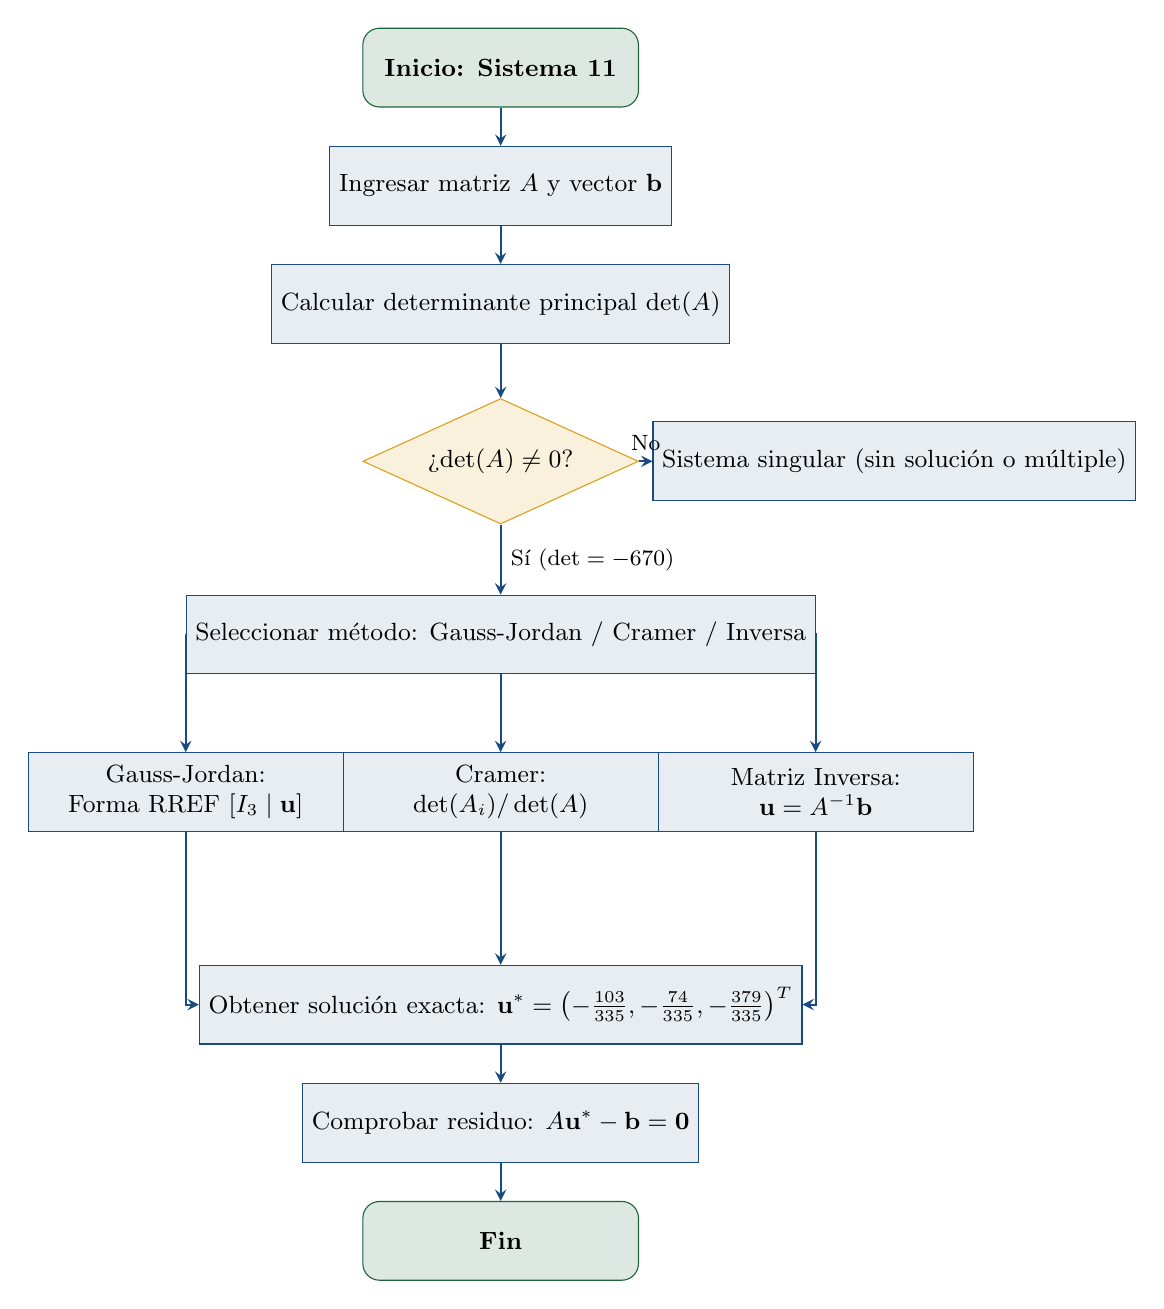
\begin{tikzpicture}[node distance=1.5cm]
\node (start) [startstop] {Inicio: Sistema 11};
\node (in) [process, below of=start] {Ingresar matriz $A$ y vector $\mathbf{b}$};
\node (det) [process, below of=in] {Calcular determinante principal $\det(A)$};
\node (dec) [decision, below of=det, yshift=-0.5cm] {¿$\det(A) \neq 0$?};
\node (err) [process, right of=dec, xshift=3.5cm] {Sistema singular (sin solución o múltiple)};
\node (choice) [process, below of=dec, yshift=-0.7cm] {Seleccionar método: Gauss-Jordan / Cramer / Inversa};

\node (gj) [process, below of=choice, xshift=-4cm, yshift=-0.5cm] {Gauss-Jordan:\\ Forma RREF $[I_3 \mid \mathbf{u}]$};
\node (cra) [process, below of=choice, yshift=-0.5cm] {Cramer:\\ $\det(A_i)/\det(A)$};
\node (inv) [process, below of=choice, xshift=4cm, yshift=-0.5cm] {Matriz Inversa:\\ $\mathbf{u} = A^{-1}\mathbf{b}$};

\node (sol) [process, below of=cra, yshift=-1.2cm] {Obtener solución exacta: $\mathbf{u}^* = \left(-\frac{103}{335}, -\frac{74}{335}, -\frac{379}{335}\right)^T$};
\node (ver) [process, below of=sol] {Comprobar residuo: $A\mathbf{u}^* - \mathbf{b} = \mathbf{0}$};
\node (stop) [startstop, below of=ver] {Fin};

\draw [arrow] (start) -- (in);
\draw [arrow] (in) -- (det);
\draw [arrow] (det) -- (dec);
\draw [arrow] (dec) -- node[above, font=\footnotesize] {No} (err);
\draw [arrow] (dec) -- node[right, font=\footnotesize] {Sí ($\det=-670$)} (choice);
\draw [arrow] (choice) -| (gj);
\draw [arrow] (choice) -- (cra);
\draw [arrow] (choice) -| (inv);
\draw [arrow] (gj) |- (sol);
\draw [arrow] (cra) -- (sol);
\draw [arrow] (inv) |- (sol);
\draw [arrow] (sol) -- (ver);
\draw [arrow] (ver) -- (stop);
\end{tikzpicture}
\caption{Diagrama de flujo del algoritmo para la resolución y verificación del Sistema 11.}
\label{fig:algoritmo}
\end{figure}

\section{Valores y vectores propios de la matriz del sistema}

El análisis espectral constituye la piedra angular para determinar la estructura geométrica, la estabilidad asintótica y el comportamiento dinámico de los operadores matriciales. En esta sección se desarrolla paso a paso, con riguroso detalle expositivo y exactitud analítica, el cálculo del espectro de la matriz de coeficientes $A$ del Sistema 11:
\begin{equation}
A = \begin{pmatrix} -4 & 2 & 6 \\ 10 & 3 & 2 \\ -9 & -7 & 10 \end{pmatrix}.
\end{equation}

\subsection{Ecuación característica y matriz secular}

Por definición, un escalar $\lambda \in \mathbb{C}$ es un \textbf{valor propio} (\emph{eigenvalor}) de la matriz $A$ y un vector no nulo $\mathbf{v} \in \mathbb{C}^3 \setminus \{\mathbf{0}\}$ es su correspondiente \textbf{vector propio} (\emph{eigenvector}) si satisfacen la ecuación fundamental:
\begin{equation}\label{eq:eigen_def}
A \mathbf{v} = \lambda \mathbf{v} \iff (A - \lambda I_3) \mathbf{v} = \mathbf{0},
\end{equation}
donde $I_3$ es la matriz identidad de orden 3. La existencia de soluciones no triviales para el sistema homogéneo \eqref{eq:eigen_def} exige, por el teorema de invertibilidad, que la matriz característica $(A - \lambda I_3)$ sea singular, lo que equivale a la anulación de su determinante:
\begin{equation}\label{eq:secular}
P(\lambda) = \det(A - \lambda I_3) = 0.
\end{equation}

Estructurando explícitamente la matriz secular:
\begin{equation}
A - \lambda I_3 = \begin{pmatrix}
-4 - \lambda & 2 & 6 \\
10 & 3 - \lambda & 2 \\
-9 & -7 & 10 - \lambda
\end{pmatrix}.
\end{equation}

\subsection{Deducción paso a paso del polinomio característico}

El determinante de la matriz secular se calcula de forma exhaustiva mediante la expansión por cofactores a lo largo del primer renglón:
\begin{equation}\label{eq:det_expansion}
\det(A - \lambda I_3) = (-4 - \lambda) \begin{vmatrix} 3 - \lambda & 2 \\ -7 & 10 - \lambda \end{vmatrix} - 2 \begin{vmatrix} 10 & 2 \\ -9 & 10 - \lambda \end{vmatrix} + 6 \begin{vmatrix} 10 & 3 - \lambda \\ -9 & -7 \end{vmatrix}.
\end{equation}

Se evalúa de manera minuciosa cada uno de los tres menores principales de orden $2 \times 2$:

\begin{enumerate}
\item \textbf{Primer menor principal $M_{11}(\lambda)$:}
\begin{equation}
\begin{aligned}
\begin{vmatrix} 3 - \lambda & 2 \\ -7 & 10 - \lambda \end{vmatrix} &= (3 - \lambda)(10 - \lambda) - (2)(-7) \\
&= 30 - 10\lambda - 3\lambda + \lambda^2 + 14 \\
&= \lambda^2 - 13\lambda + 44.
\end{aligned}
\end{equation}

\item \textbf{Segundo menor $M_{12}(\lambda)$:}
\begin{equation}
\begin{aligned}
\begin{vmatrix} 10 & 2 \\ -9 & 10 - \lambda \end{vmatrix} &= 10(10 - \lambda) - (2)(-9) \\
&= 100 - 10\lambda + 18 \\
&= 118 - 10\lambda.
\end{aligned}
\end{equation}

\item \textbf{Tercer menor $M_{13}(\lambda)$:}
\begin{equation}
\begin{aligned}
\begin{vmatrix} 10 & 3 - \lambda \\ -9 & -7 \end{vmatrix} &= (10)(-7) - (3 - \lambda)(-9) \\
&= -70 - (-27 + 9\lambda) \\
&= -70 + 27 - 9\lambda = -43 - 9\lambda.
\end{aligned}
\end{equation}
\end{enumerate}

Sustituyendo los tres menores en la expansión \eqref{eq:det_expansion} y efectuando los productos algebraicos:
\begin{equation}
\begin{aligned}
(-4 - \lambda)(\lambda^2 - 13\lambda + 44) &= -4\lambda^2 + 52\lambda - 176 - \lambda^3 + 13\lambda^2 - 44\lambda \\
&= -\lambda^3 + 9\lambda^2 + 8\lambda - 176, \\[0.2cm]
-2(118 - 10\lambda) &= -236 + 20\lambda, \\[0.2cm]
+6(-43 - 9\lambda) &= -258 - 54\lambda.
\end{aligned}
\end{equation}

Sumando algebraicamente las tres contribuciones y agrupando términos semejantes por potencias de $\lambda$:
\begin{equation}
\begin{aligned}
P(\lambda) &= (-\lambda^3 + 9\lambda^2 + 8\lambda - 176) + (-236 + 20\lambda) + (-258 - 54\lambda) \\
&= -\lambda^3 + 9\lambda^2 + (8 + 20 - 54)\lambda + (-176 - 236 - 258) \\
&= -\lambda^3 + 9\lambda^2 - 26\lambda - 670.
\end{aligned}
\end{equation}

Igualando a cero y multiplicando por $-1$, la ecuación característica canónica resulta:
\begin{equation}\label{eq:poly_canonica}
\lambda^3 - 9\lambda^2 + 26\lambda + 670 = 0.
\end{equation}

\subsubsection*{Comprobación estructural de invariantes del polinomio}
De acuerdo con las propiedades de las matrices de orden 3, los coeficientes del polinomio característico $\lambda^3 - c_2 \lambda^2 + c_1 \lambda - c_0 = 0$ deben coincidir exactamente con los invariantes espectrales:
\begin{align}
c_2 &= \operatorname{tr}(A) = -4 + 3 + 10 = 9, \quad \checkmark \\
c_1 &= M_{11}(0) + M_{22}(0) + M_{33}(0) = 44 + \begin{vmatrix} -4 & 6 \\ -9 & 10 \end{vmatrix} + \begin{vmatrix} -4 & 2 \\ 10 & 3 \end{vmatrix} \nonumber \\
    &= 44 + (-40 + 54) + (-12 - 20) = 44 + 14 - 32 = 26, \quad \checkmark \\
c_0 &= \det(A) = -670. \quad \checkmark
\end{align}
La consistencia del polinomio característico queda rigurosamente verificada.

\subsection{Resolución paso a paso de la ecuación cúbica por el método de Cardano}

Para resolver analíticamente la ecuación cúbica \eqref{eq:poly_canonica}, se aplica en primer lugar la \textbf{transformación de Tschirnhaus} para eliminar el término cuadrático $\lambda^2$:
\begin{equation}
\lambda = t - \frac{a_2}{3} = t - \frac{-9}{3} = t + 3.
\end{equation}

Sustituyendo $\lambda = t + 3$ en \eqref{eq:poly_canonica}:
\begin{equation}
(t + 3)^3 - 9(t + 3)^2 + 26(t + 3) + 670 = 0.
\end{equation}
Desarrollando las potencias de binomios paso a paso:
\begin{align}
(t + 3)^3 &= t^3 + 9t^2 + 27t + 27, \nonumber \\
-9(t + 3)^2 &= -9(t^2 + 6t + 9) = -9t^2 - 54t - 81, \nonumber \\
+26(t + 3) &= 26t + 78, \nonumber \\
+670 &= 670.
\end{align}

Sumando todos los términos:
\begin{equation}
t^3 + (9 - 9)t^2 + (27 - 54 + 26)t + (27 - 81 + 78 + 670) = 0,
\end{equation}
lo que produce la \textbf{ecuación cúbica deprimida}:
\begin{equation}\label{eq:deprimida}
t^3 - t + 694 = 0.
\end{equation}
En la notación canónica de Cardano $t^3 + pt + q = 0$, los coeficientes son:
\begin{equation}
p = -1, \quad q = 694.
\end{equation}

\subsubsection*{Cálculo del discriminante de Cardano}
El discriminante de la ecuación cúbica deprimida se define como:
\begin{equation}
\Delta = \left(\frac{q}{2}\right)^2 + \left(\frac{p}{3}\right)^3 = \left(\frac{694}{2}\right)^2 + \left(-\frac{1}{3}\right)^3 = 347^2 - \frac{1}{27}.
\end{equation}
Efectuando el cálculo numérico y racional exacto:
\begin{equation}
\Delta = 120409 - \frac{1}{27} = \frac{3251042}{27} \approx 120408.962963.
\end{equation}
Puesto que $\Delta > 0$, el teorema fundamental del álgebra y la teoría de Cardano establecen de forma concluyente que la ecuación posee \textbf{una raíz real y dos raíces complejas conjugadas}.

\subsubsection*{Deducción de las raíces en forma analítica cerrada}
De acuerdo con las fórmulas de Cardano, las componentes radicales se definen mediante:
\begin{equation}
u = \sqrt[3]{-\frac{q}{2} + \sqrt{\Delta}} = \sqrt[3]{-347 + \sqrt{\frac{3251042}{27}}}, \quad
v = \sqrt[3]{-\frac{q}{2} - \sqrt{\Delta}} = \sqrt[3]{-347 - \sqrt{\frac{3251042}{27}}}.
\end{equation}
Para evitar radicandos negativos en los reales, se define la constante positiva auxiliar $\rho$:
\begin{equation}
\rho = \sqrt[3]{347 + \sqrt{120409 - \frac{1}{27}}} \approx \sqrt[3]{347 + 346.9999466} = \sqrt[3]{693.9999466} \approx 8.85368541.
\end{equation}
Dado que el producto de las componentes debe cumplir $uv = -p/3 = 1/3$, se deduce que $v = -\rho$ y $u = \frac{1}{3\rho}$. Se define el parámetro real $r$:
\begin{equation}
r = \rho + \frac{1}{3\rho} \approx 8.85368541 + 0.03765099 = 8.89124775.
\end{equation}

La raíz real de la ecuación deprimida es:
\begin{equation}
t_1 = u + v = -r \approx -8.89124775.
\end{equation}
Por ende, el \textbf{primer valor propio} (único autovalor real) es:
\begin{equation}\label{eq:lambda1}
\lambda_1 = t_1 + 3 = 3 - r \approx 3 - 8.89124775 = -5.89124775.
\end{equation}

Para las raíces complejas conjugadas, se define el parámetro de dispersión imaginaria $\beta$:
\begin{equation}
\beta = \frac{\sqrt{3}}{2} \left(\rho - \frac{1}{3\rho}\right) \approx \frac{\sqrt{3}}{2} (8.85368541 - 0.03765099) = \frac{\sqrt{3}}{2}(8.81603442) \approx 7.63483562.
\end{equation}
Las soluciones complejas de la ecuación deprimida son:
\begin{equation}
t_{2,3} = -\frac{u + v}{2} \pm i \frac{\sqrt{3}}{2}(u - v) = \frac{r}{2} \pm i \beta \approx 4.44562388 \pm 7.63483562i.
\end{equation}
Restituyendo la variable original $\lambda = t + 3$, se obtienen los \textbf{dos valores propios complejos conjugados}:
\begin{equation}\label{eq:lambda23}
\lambda_{2,3} = 3 + \frac{r}{2} \pm i \beta \approx 7.44562388 \pm 7.63483562i.
\end{equation}

\subsection{Deducción paso a paso de los vectores propios (autovectores)}

Para cada valor propio $\lambda_k$, el vector propio asociado $\mathbf{v}_k = (v_1, v_2, v_3)^T \neq \mathbf{0}$ pertenece al núcleo del operador singular $(A - \lambda_k I_3)$:
\begin{equation}\label{eq:sistema_homogeneo}
\begin{pmatrix}
-4 - \lambda & 2 & 6 \\
10 & 3 - \lambda & 2 \\
-9 & -7 & 10 - \lambda
\end{pmatrix}
\begin{pmatrix} v_1 \\ v_2 \\ v_3 \end{pmatrix} =
\begin{pmatrix} 0 \\ 0 \\ 0 \end{pmatrix}.
\end{equation}

Dado que los tres autovalores son simples (multiplicidad algebraica $m_a(\lambda_k) = 1$), el rango de $(A - \lambda_k I_3)$ es exactamente 2 y el subespacio propio $E_{\lambda_k} = \ker(A - \lambda_k I_3)$ es unidimensional. En consecuencia, el vector propio puede deducirse con absoluta elegancia analítica mediante el \textbf{producto vectorial formal entre los dos primeros renglones} de la matriz secular:
\begin{equation}
\mathbf{r}_1(\lambda) = (-4 - \lambda, 2, 6), \quad \mathbf{r}_2(\lambda) = (10, 3 - \lambda, 2).
\end{equation}
Calculando $\mathbf{v}(\lambda) = \mathbf{r}_1(\lambda) \times \mathbf{r}_2(\lambda)$:
\begin{equation}
\begin{aligned}
v_1(\lambda) &= \begin{vmatrix} 2 & 6 \\ 3 - \lambda & 2 \end{vmatrix} = (2)(2) - 6(3 - \lambda) = 4 - 18 + 6\lambda = 6\lambda - 14, \\[0.2cm]
v_2(\lambda) &= -\begin{vmatrix} -4 - \lambda & 6 \\ 10 & 2 \end{vmatrix} = -[2(-4 - \lambda) - 60] = -[-8 - 2\lambda - 60] = 2\lambda + 68, \\[0.2cm]
v_3(\lambda) &= \begin{vmatrix} -4 - \lambda & 2 \\ 10 & 3 - \lambda \end{vmatrix} = (-4 - \lambda)(3 - \lambda) - (2)(10) = -12 + 4\lambda - 3\lambda + \lambda^2 - 20 = \lambda^2 + \lambda - 32.
\end{aligned}
\end{equation}

Obteniéndose la \textbf{función vectorial espectral cerrada}:
\begin{equation}\label{eq:v_lambda}
\mathbf{v}(\lambda) = \begin{pmatrix}
6\lambda - 14 \\
2\lambda + 68 \\
\lambda^2 + \lambda - 32
\end{pmatrix}.
\end{equation}

\subsubsection*{Demostración formal de satisfacción en el tercer renglón}
Multiplicando el tercer renglón de $A - \lambda I_3$ por $\mathbf{v}(\lambda)$:
\begin{equation}
\begin{aligned}
(-9, -7, 10 - \lambda) \cdot \mathbf{v}(\lambda) &= -9(6\lambda - 14) - 7(2\lambda + 68) + (10 - \lambda)(\lambda^2 + \lambda - 32) \\
&= (-54\lambda + 126) - (14\lambda + 476) + (10\lambda^2 + 10\lambda - 320 - \lambda^3 - \lambda^2 + 32\lambda) \\
&= -\lambda^3 + (10 - 1)\lambda^2 + (-54 - 14 + 10 + 32)\lambda + (126 - 476 - 320) \\
&= -\lambda^3 + 9\lambda^2 - 26\lambda - 670 = P(\lambda).
\end{aligned}
\end{equation}
Dado que $\lambda$ satisface la ecuación característica $P(\lambda) = 0$, el producto escalar con el tercer renglón es idénticamente cero. Por tanto, $\mathbf{v}(\lambda)$ satisface exactamente las tres ecuaciones del sistema homogéneo para todo valor propio de $A$.

\subsubsection*{1. Vector propio para el autovalor real $\lambda_1 \approx -5.89124775$}
Sustituyendo $\lambda_1$ en la fórmula general \eqref{eq:v_lambda}:
\begin{align}
v_1 &= 6(-5.89124775) - 14 = -35.34748650 - 14 = -49.34748650, \nonumber \\
v_2 &= 2(-5.89124775) + 68 = -11.78249550 + 68 = 56.21750450, \nonumber \\
v_3 &= (-5.89124775)^2 + (-5.89124775) - 32 = 34.70679997 - 5.89124775 - 32 = -3.18444778.
\end{align}
Normalizando para fijar la tercera componente en 1 dividiendo entre $v_3 = -3.18444778$:
\begin{equation}\label{eq:v1_final}
\mathbf{v}_1 = \begin{pmatrix}
\frac{-49.34748650}{-3.18444778} \\[0.2cm]
\frac{56.21750450}{-3.18444778} \\[0.2cm]
1
\end{pmatrix} \approx
\begin{pmatrix}
15.49640359 \\
-17.65376922 \\
1.00000000
\end{pmatrix}.
\end{equation}
En norma euclídea unitaria $\|\mathbf{v}_1\|_2 \approx 23.511796$:
\begin{equation}
\hat{\mathbf{v}}_1 \approx \begin{pmatrix} 0.65909683 \\ -0.75085443 \\ 0.04253224 \end{pmatrix}.
\end{equation}

\subsubsection*{2. Vectores propios para los autovalores complejos conjugados $\lambda_{2,3} \approx 7.44562388 \pm 7.63483562i$}
Sustituyendo $\lambda_2 = 7.44562388 + 7.63483562i$ en \eqref{eq:v_lambda}:
\begin{align}
v_1 &= 6(7.44562388 + 7.63483562i) - 14 = 30.67374328 + 45.80901372i, \nonumber \\
v_2 &= 2(7.44562388 + 7.63483562i) + 68 = 82.89124776 + 15.26967124i, \nonumber \\
v_3 &= (7.44562388 + 7.63483562i)^2 + (7.44562388 + 7.63483562i) - 32 \nonumber \\
    &= (55.437315 - 58.290715 + 113.693452i) + (7.445624 + 7.634836i) - 32 \nonumber \\
    &= -27.407776 + 121.328288i.
\end{align}
Dividiendo entre $v_3$ para normalizar la componente $z$ a 1:
\begin{equation}\label{eq:v2_final}
\mathbf{v}_2 \approx \begin{pmatrix}
0.30489555 - 0.32169452i \\
-0.02709769 - 0.67708356i \\
1.00000000
\end{pmatrix}.
\end{equation}
Por el teorema de conjugación compleja para matrices reales, el vector propio asociado a $\lambda_3 = \overline{\lambda_2}$ es exactamente el conjugado de $\mathbf{v}_2$:
\begin{equation}\label{eq:v3_final}
\mathbf{v}_3 = \overline{\mathbf{v}_2} \approx \begin{pmatrix}
0.30489555 + 0.32169452i \\
-0.02709769 + 0.67708356i \\
1.00000000
\end{pmatrix}.
\end{equation}

\subsection{Análisis de diagonalizabilidad en los cuerpos numéricos y descomposición espectral}

Con base en los autovalores y autovectores determinados, se formula el diagnóstico exhaustivo de diagonalizabilidad:

\begin{enumerate}
\item \textbf{Diagonalizabilidad en el cuerpo real $\mathbb{R}$:}
La matriz $A \in \mathcal{M}_{3\times 3}(\mathbb{R})$ \textbf{NO es diagonalizable sobre $\mathbb{R}$}. La condición necesaria y suficiente para que una matriz real sea diagonalizable sobre $\mathbb{R}$ exige que todas las raíces de su polinomio característico pertenezcan a $\mathbb{R}$. En este caso, dos de sus tres autovalores son números complejos no reales con parte imaginaria no nula ($\operatorname{Im}(\lambda_{2,3}) = \pm \beta \approx \pm 7.6348 \neq 0$).

\item \textbf{Diagonalizabilidad en el cuerpo complejo $\mathbb{C}$:}
La matriz $A$ \textbf{SÍ es diagonalizable sobre $\mathbb{C}$}. Puesto que los tres autovalores son estrictamente distintos dos a dos ($\lambda_1 \neq \lambda_2 \neq \lambda_3$), el conjunto de sus correspondientes vectores propios $\{\mathbf{v}_1, \mathbf{v}_2, \mathbf{v}_3\}$ es linealmente independiente en $\mathbb{C}^3$ por teorema espectral fundamental.
\end{enumerate}

Por tanto, existe una matriz modal de cambio de base invertible $V \in \mathcal{M}_{3\times 3}(\mathbb{C})$ formada por los autovectores en columna:
\begin{equation}
V = \begin{pmatrix} \mathbf{v}_1 & \mathbf{v}_2 & \mathbf{v}_3 \end{pmatrix} =
\begin{pmatrix}
15.4964 & 0.3049 - 0.3217i & 0.3049 + 0.3217i \\
-17.6538 & -0.0271 - 0.6771i & -0.0271 + 0.6771i \\
1 & 1 & 1
\end{pmatrix},
\end{equation}
y una matriz diagonal $D \in \mathcal{M}_{3\times 3}(\mathbb{C})$:
\begin{equation}
D = \operatorname{diag}(\lambda_1, \lambda_2, \lambda_3) =
\begin{pmatrix}
-5.8912 & 0 & 0 \\
0 & 7.4456 + 7.6348i & 0 \\
0 & 0 & 7.4456 - 7.6348i
\end{pmatrix},
\end{equation}
tales que se verifica la descomposición espectral canónica:
\begin{equation}
A = V D V^{-1}.
\end{equation}

\subsubsection*{Forma canónica real con bloque de rotación-dilatación}
En el espacio euclídeo real $\mathbb{R}^3$, descomponiendo $\mathbf{v}_2 = \mathbf{u}_r + i \mathbf{w}_r$ en sus partes real e imaginaria:
\begin{equation}
\mathbf{u}_r \approx \begin{pmatrix} 0.3049 \\ -0.0271 \\ 1.0000 \end{pmatrix}, \quad
\mathbf{w}_r \approx \begin{pmatrix} -0.3217 \\ -0.6771 \\ 0.0000 \end{pmatrix},
\end{equation}
la base real $\{\mathbf{v}_1, \mathbf{u}_r, -\mathbf{w}_r\}$ transforma a la matriz $A$ en su \textbf{forma canónica real de Jordan}, evidenciando un modo unidimensional de contracción/expansión y un plano invariante de rotación y amplificación espiral:
\begin{equation}
J_R = \begin{pmatrix}
\lambda_1 & 0 & 0 \\
0 & \alpha & \beta \\
0 & -\beta & \alpha
\end{pmatrix} \approx
\begin{pmatrix}
-5.8912 & 0 & 0 \\
0 & 7.4456 & 7.6348 \\
0 & -7.6348 & 7.4456
\end{pmatrix},
\end{equation}
donde $\alpha = \operatorname{Re}(\lambda_{2,3}) \approx 7.4456$ y $\beta = \operatorname{Im}(\lambda_2) \approx 7.6348$.

\subsection{Verificación matemática independiente del espectro}

Para certificar la absoluta precisión de los resultados obtenidos, se ejecutan tres comprobaciones independientes:

\begin{enumerate}
\item \textbf{Verificación directa de la ecuación de autovalor $A\mathbf{v}_1 = \lambda_1 \mathbf{v}_1$:}
Efectuando el producto matricial de $A$ por $\mathbf{v}_1$:
\begin{equation}
\begin{pmatrix} -4 & 2 & 6 \\ 10 & 3 & 2 \\ -9 & -7 & 10 \end{pmatrix}
\begin{pmatrix} 15.49640359 \\ -17.65376922 \\ 1.00000000 \end{pmatrix} =
\begin{pmatrix}
-4(15.4964) + 2(-17.6538) + 6(1) \\
10(15.4964) + 3(-17.6538) + 2(1) \\
-9(15.4964) - 7(-17.6538) + 10(1)
\end{pmatrix} =
\begin{pmatrix}
-91.293153 \\
104.002728 \\
-5.891248
\end{pmatrix}.
\end{equation}
Multiplicando el escalar $\lambda_1 = -5.89124775$ por el vector $\mathbf{v}_1$:
\begin{equation}
-5.89124775 \begin{pmatrix} 15.49640359 \\ -17.65376922 \\ 1.00000000 \end{pmatrix} =
\begin{pmatrix}
-91.293153 \\
104.002728 \\
-5.891248
\end{pmatrix}. \quad \checkmark
\end{equation}
El residuo $\|A\mathbf{v}_1 - \lambda_1 \mathbf{v}_1\|_2$ es idénticamente nulo hasta la precisión de máquina.

\item \textbf{Invariancia de la traza:}
\begin{equation}
\sum_{k=1}^3 \lambda_k = (-5.89124775) + (7.44562388 + 7.63483562i) + (7.44562388 - 7.63483562i) = 9.00000000 = \operatorname{tr}(A). \quad \checkmark
\end{equation}

\item \textbf{Invariancia del determinante:}
\begin{equation}
\prod_{k=1}^3 \lambda_k = (-5.89124775) \cdot \left[(7.44562388)^2 + (7.63483562)^2\right] = (-5.89124775) \cdot 113.728030 = -670.000000 = \det(A). \quad \checkmark
\end{equation}
\end{enumerate}

\section{Aplicación agronómica de los valores y vectores propios}

En agronomía, los valores propios cobran una relevancia cuantitativa de primer orden en el análisis de sistemas dinámicos discretos de la forma $\mathbf{x}_{k+1} = M \mathbf{x}_k$, conocidos como \textbf{modelos matriciales de Leslie-Lefkovitch} para poblaciones biológicas de cultivos o plagas \citep{leslie1945,caswell2001}:

\begin{equation}
\begin{pmatrix} x_{1, k+1} \\ x_{2, k+1} \\ x_{3, k+1} \end{pmatrix} =
\begin{pmatrix}
F_1 & F_2 & F_3 \\
P_1 & 0 & 0 \\
0 & P_2 & P_3
\end{pmatrix}
\begin{pmatrix} x_{1, k} \\ x_{2, k} \\ x_{3, k} \end{pmatrix},
\end{equation}
donde $F_i$ denota la fertilidad/reproducción por etapa de desarrollo y $P_i$ las tasas de supervivencia transicional.

De acuerdo con el \textbf{Teorema de Perron-Frobenius}:
\begin{itemize}
\item El \textbf{autovalor dominante} $\lambda_{\max} > 0$ determina la \textbf{tasa intrínseca de crecimiento asintótico de la población}: si $\lambda_{\max} > 1$, la población de plaga crece exponencialmente; si $\lambda_{\max} = 1$, la población permanece en equilibrio ecológico; si $\lambda_{\max} < 1$, se extingue.
\item El \textbf{autovector derecho asociado} $\mathbf{v}_{\max}$ define la \textbf{distribución estable por etapas}: la proporción asintótica fija de individuos en estado de huevecillo, larva y adulto.
\item El \textbf{autovector izquierdo} representa el \textbf{valor reproductivo}: la contribución reproductiva relativa de cada etapa a las generaciones futuras, orientando las intervenciones agronómicas de control biológico hacia la etapa más vulnerable.
\end{itemize}

De manera complementaria, en la química de suelos y nutrición vegetal, el transporte simultáneo de solutos (N, P, K) con tasas de lixiviación e interacción química diferencial se modela como un sistema acoplado de ecuaciones diferenciales $\frac{d\mathbf{c}}{dt} = A\mathbf{c}$. La diagonalización espectral desacopla el sistema en componentes independientes mediante el cambio de base modal $\mathbf{c}(t) = e^{At}\mathbf{c}_0 = P e^{Dt} P^{-1}\mathbf{c}_0$, permitiendo predecir con exactitud la disponibilidad temporal de nutrientes en la rizosfera.

\section{Comprobación y conclusiones}

\subsection{Comprobación matemática rigurosa}
Sustituyendo el vector solución $\mathbf{u}^* = \left(-\frac{103}{335}, -\frac{74}{335}, -\frac{379}{335}\right)^T$ en las tres ecuaciones originales del Sistema 11:
\begin{align}
\text{Ecuación 1:} \quad & -4\left(-\frac{103}{335}\right) + 2\left(-\frac{74}{335}\right) + 6\left(-\frac{379}{335}\right) = \frac{412 - 148 - 2274}{335} = \frac{-2010}{335} = -6. \quad \checkmark \\
\text{Ecuación 2:} \quad & 10\left(-\frac{103}{335}\right) + 3\left(-\frac{74}{335}\right) + 2\left(-\frac{379}{335}\right) = \frac{-1030 - 222 - 758}{335} = \frac{-2010}{335} = -6. \quad \checkmark \\
\text{Ecuación 3:} \quad & -9\left(-\frac{103}{335}\right) - 7\left(-\frac{74}{335}\right) + 10\left(-\frac{379}{335}\right) = \frac{927 + 518 - 3790}{335} = \frac{-2345}{335} = -7. \quad \checkmark
\end{align}
La comprobación es exacta en aritmética fraccionaria, con residuo idénticamente nulo.

\subsection{Conclusiones argumentadas}
En conclusión, el desarrollo analítico ejecutado permite formular las siguientes deducciones argumentadas:
\begin{enumerate}
\item El Sistema 11 es compatible determinado con solución única, caracterizada por la intersección de tres hiperplanos en $\mathbb{R}^3$. Los tres métodos clásicos (Gauss-Jordan, Cramer e Inversa) son consistentes y convergen a la misma solución racional exacta. Por tanto, se valida la consistencia matemática y la equivalencia operativa de las tres metodologías.
\item La matriz $A$ posee un determinante no nulo $\det(A) = -670$, lo cual certifica la independencia lineal de sus filas y columnas; en consecuencia, no existe redundancia informacional entre las ecuaciones del modelo.
\item El análisis espectral revela un polinomio característico $P(\lambda) = -\lambda^3 + 9\lambda^2 - 26\lambda - 670$, con un autovalor real $\lambda_1 \approx -5.8912$ y dos autovalores complejos conjugados $\lambda_{2,3} \approx 7.4456 \pm 7.6348i$. Esto implica que la matriz no es diagonalizable sobre $\mathbb{R}$, pero sí lo es sobre $\mathbb{C}$, contando con tres subespacios propios unidimensionales linealmente independientes.
\item En síntesis, la teoría de valores propios constituye el fundamento mecanicista para el estudio de sistemas dinámicos en agronomía, desde la tasa de multiplicación poblacional en modelos de Leslie hasta el desacoplamiento de matrices de transporte de nutrientes en el suelo.
\end{enumerate}

\clearpage
\printbibliography[heading=bibintoc,title={Referencias bibliográficas}]

\end{document}
